\chapter{Introduction}\label{chapter:introduction}

\textbf{Locking mechanism is important.}
In modern computing environments, the efficiency of locking mechanisms plays a crucial role in the performance of various systems, including databases~\parencite{lomet1993key, graefe2007hierarchical}, file systems~\parencite{lee2021concurrent, gao2023citron, lee2019write}, and operating systems~\parencite{readerWriterLocks2017, mmapSem2017}. As these systems grow in scale and complexity, the demand for more sophisticated and efficient locking mechanisms becomes crucial. One of the fundamental challenges in this context is managing concurrent access to shared resources. Traditional locking techniques, such as single-lock mechanisms, often lead to significant performance bottlenecks, particularly in high-concurrency scenarios.

\textbf{Range locks boot performance through resource segmentation.} 
Range lock~\parencite{gao2023citron, kogan2020scalable} provides a more refined approach to this issue by partitioning a shared resource into multiple arbitrary-sized segments. Different processes can exclusively acquire each of these segments. This strategy effectively addresses the drawbacks and bottlenecks associated with single-lock methods, significantly improving the performance.

\textbf{DBMS needs range locks.}
As database sizes increase exponentially, locking the entire database becomes impractical. This approach will prevent concurrent transactions from progressing, resulting in poor throughput and high latency. The previous key-range locking in DBMS is complex and tightly coupled with lock-based concurrency control protocols~\parencite{graefe2007hierarchical, andy2022database}. 
Consequently, this technique does not apply to general DBMS operations like variable-sized page allocation. Therefore, a new technique, such as range locks, is desirable.

\textbf{Filesystem needs range locks.}
In high-performance file systems, particularly those used in large-scale and distributed computing environments, efficiently managing concurrent access to shared files is crucial. As file systems scale to accommodate massive data sets and numerous parallel I/O operations, traditional locking mechanisms often become bottlenecks, reducing throughput and increasing latency. Range locks offer a solution by allowing multiple processes to access different file segments simultaneously without interfering with each other. This segmentation minimizes contention and improves performance by enabling finer-grained locking at the segment level. For file systems handling concurrent access to large files, especially in high-performance computing (HPC) environments, adopting range locks can significantly enhance efficiency and scalability~\parencite{gao2023citron, lee2021concurrent}.

\textbf{Operating system needs range locks.}
There has been growing interest in using range locks within the Linux kernel community. The focus is on using range locks to alleviate contention issues associated with \texttt{mmap\_sem}, a semaphore that manages access to virtual memory areas (VMAs). VMAs represent distinct sections of an application's virtual address space and are organized in a red-black tree. The \texttt{mmap\_sem} semaphore controls access for various operations such as memory mapping, unmapping, protection, and handling page faults. This becomes problematic for data-intensive applications with large, dynamically allocated memory, as contention on this semaphore can become a significant performance bottleneck.

\textbf{Existing range lock needs improvement.}
Previous implementations of range-locking mechanisms often need to improve their performance. These implementations often suffer from contention points due to the reliance on a single lock~\parencite{linuxRangeLockImpl2013, song2013parallelizing}. Additionally, some methods may be complex and tightly coupled with lock-based concurrency control protocols, which are not applicable for general DBMS operations~\parencite{graefe2007hierarchical, andy2022database}. These limitations underscore the need for more refined and scalable solutions that can better handle the demands of modern, large-scale systems.

\textbf{New concurrent range-locking design.} In this research's scope, we propose a new lock-free concurrent range-locking design. We address previous bottleneck issues by leveraging a probabilistic concurrent skip list~\parencite{herlihy2006provably, herlihy2020art} and replace traditional locking by \texttt{compare-and-swap} methods. By doing so, we address the previous range lock bottleneck issues and maintain the lock's high level of performance.

\begin{figure}[h]
    \centering
    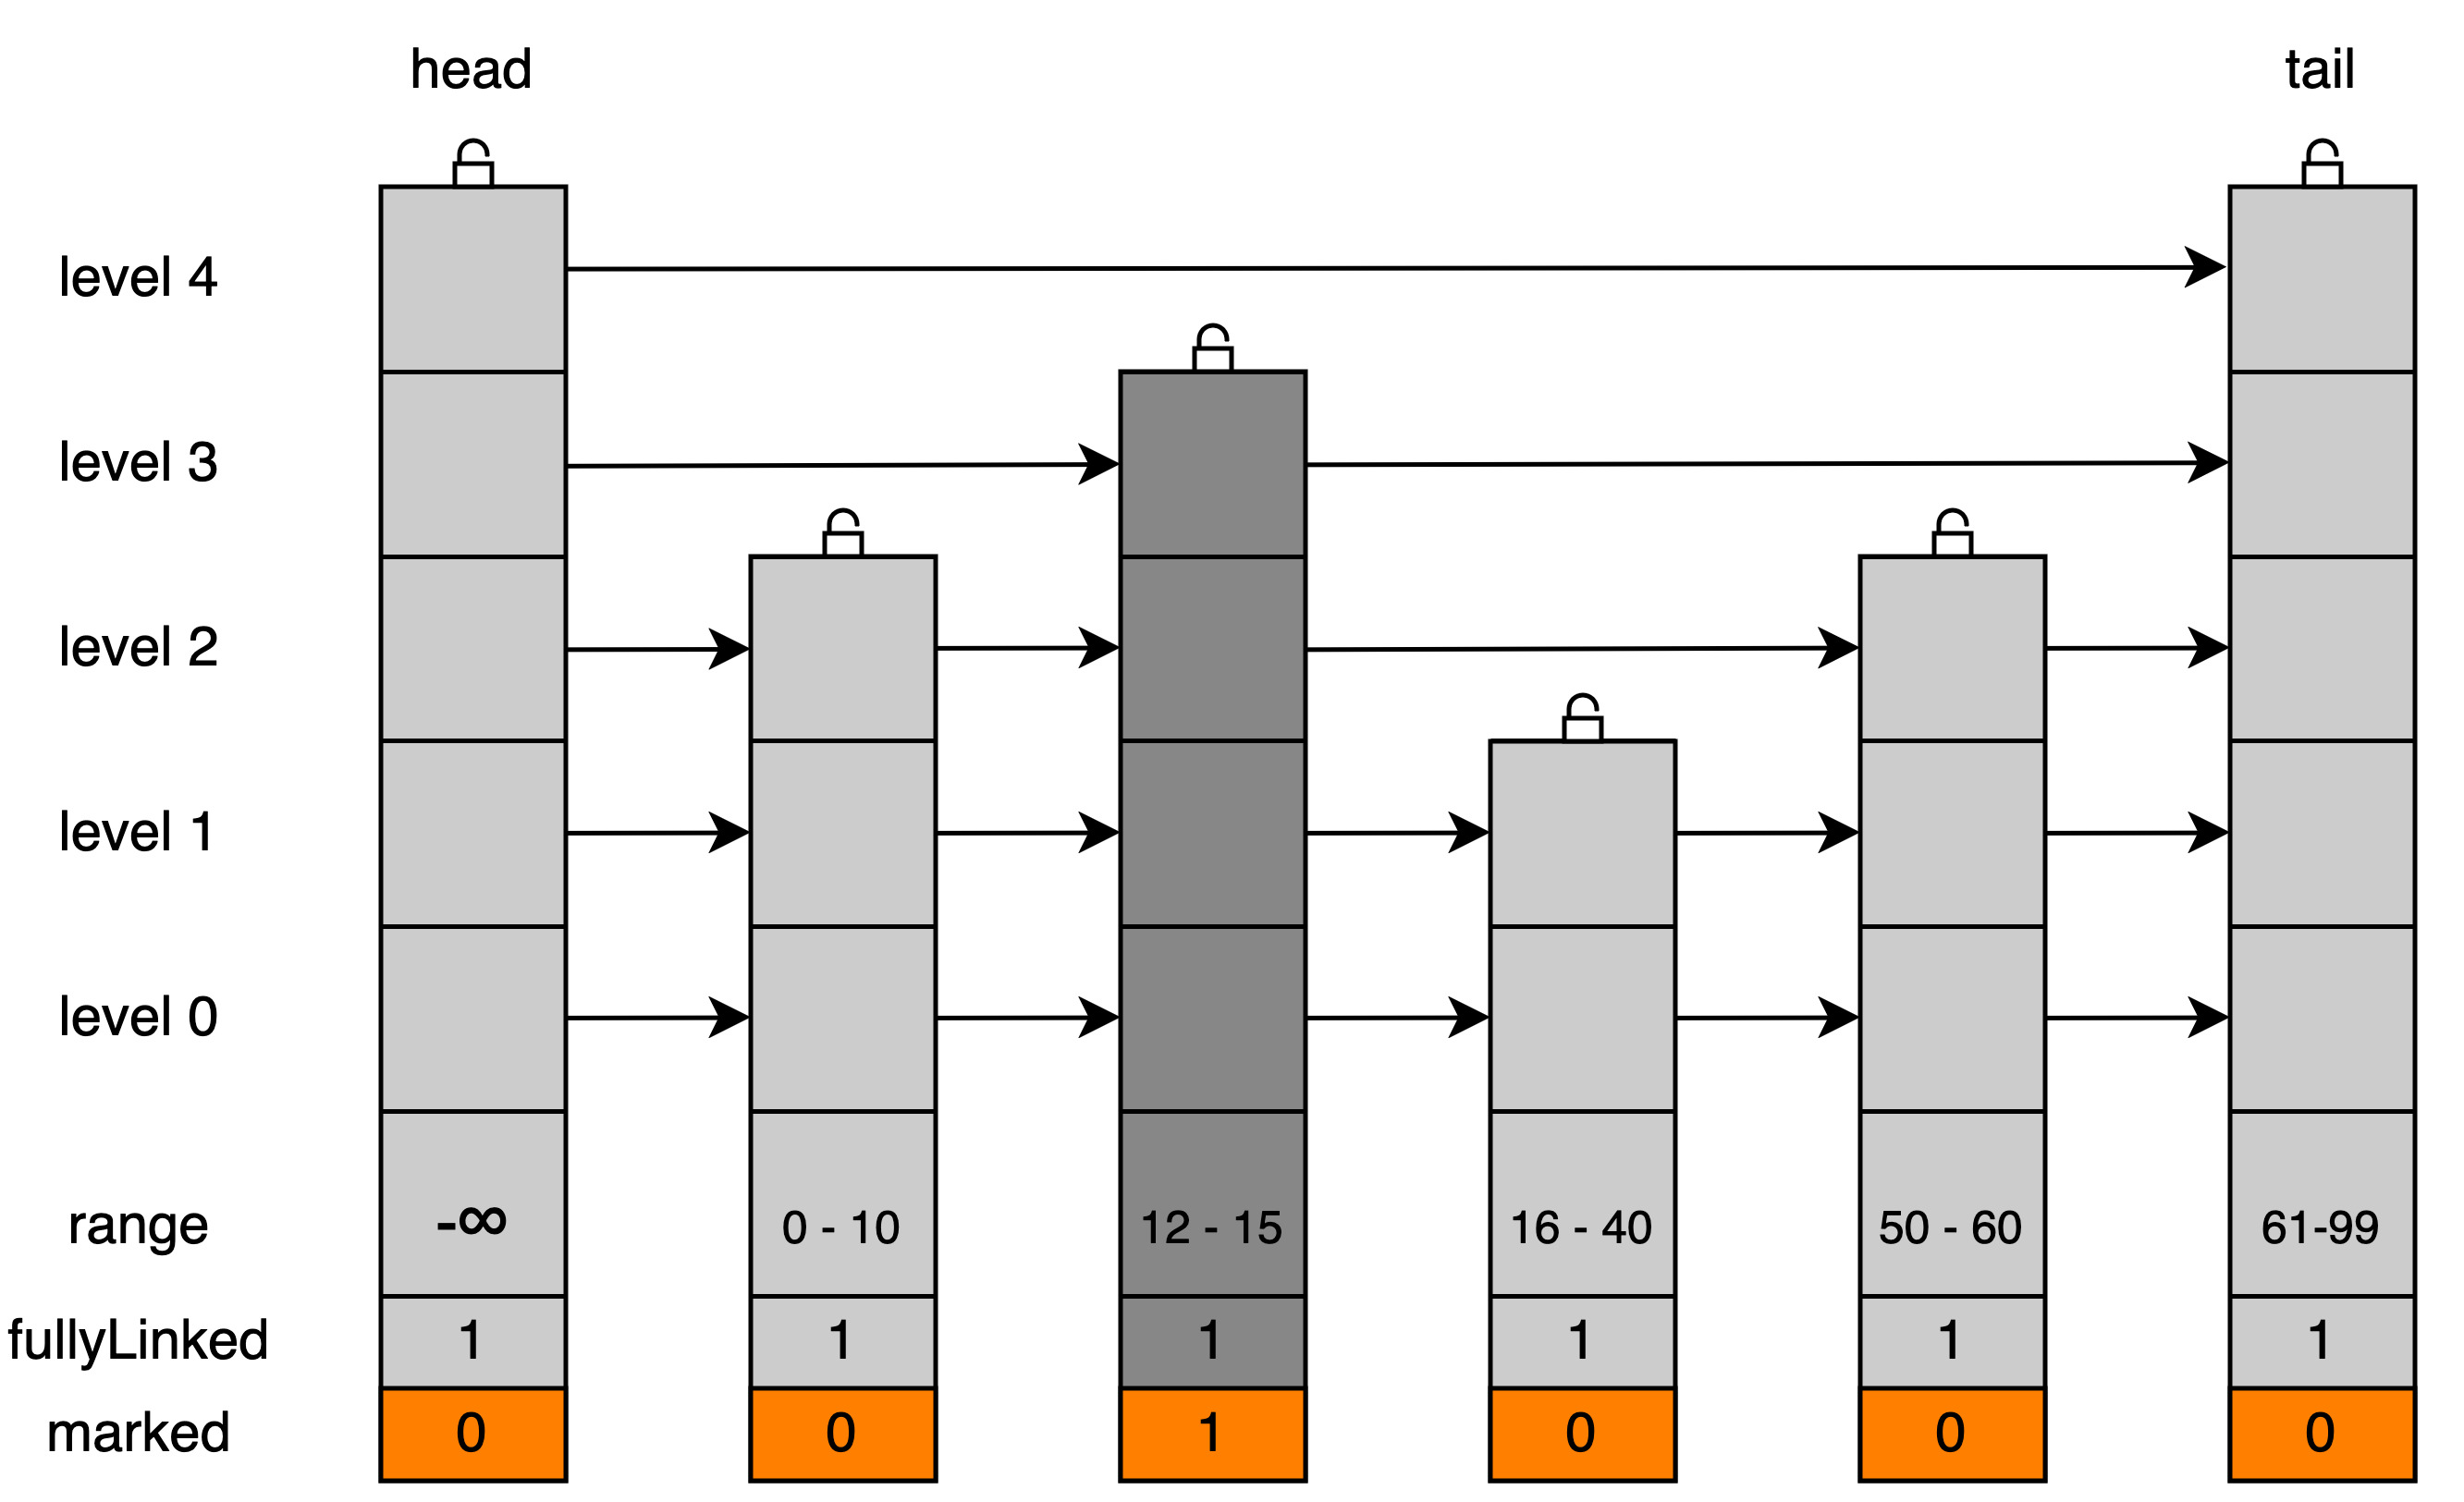
\includegraphics[width=0.8\textwidth]{./figures/concurrent_range_lock.jpg}
    \caption{Concurrent range lock}
    \label{fig:concurrent_range_lock}
\end{figure}

\textbf{Outline of the research.} The scope of this research includes developing and evaluating the proposed range-locking mechanism. We will evaluate focusing on performance under heavy concurrent accesses, ensuring the correctness of data access in overlapping ranges and concurrent operations. Additionally, we will compare the performance of the proposed solution with existing state-of-the-art approaches to provide a comprehensive assessment of its effectiveness.